
\section{Power Series and ODE}
\subsection{Higher Derivatives}
\subsubsection{Common Identities}
\begin{table}[H]
    \centering
    \renewcommand{\arraystretch}{2.2}
    \caption{Highier Derivatives Common Identities}
    \label{table:4.1}
    \begin{tabular}{|c|c|c|}\hline
       Num.&$y\bracket{x}$&$y^{\bracket{n}}\bracket{x}$\\ \hline
       1.&$x^a$&$\displaystyle\frac{a!}{\bracket{a-n}!}\cdot x^{a-n}$\\
       2.&$\displaystyle\e{ax}$&$a^n\cdot\e{ax}$\\
       3.&$\displaystyle\ln{x}$&$\displaystyle\bracket{-1}^{n-1}\cdot\frac{\bracket{n-1}!}{x^n}$\\
       4.&$\displaystyle\sinn{x}$&$\displaystyle \sinn{x+\frac{n\pi}{2}}$\\
       5.&$\displaystyle\coss{x}$&$\displaystyle \coss{x+\frac{n\pi}{2}}$\\
       6.&$\displaystyle\sinn{ax}$&$\displaystyle a^n\cdot\sinn{ax+\frac{n\pi}{2}}$\\
       7.&$\displaystyle\coss{ax}$&$\displaystyle a^n\cdot\coss{ax+\frac{n\pi}{2}}$\\
       8.&$\displaystyle\sinh\bracket{ax}$&$\displaystyle\frac{a^n}{2}\cbracket{\sbracket{1+\bracket{-1}^n}\sinh\bracket{ax}+\sbracket{1-\bracket{-1}^n}\cosh\bracket{ax}}$\\
       9.&$\displaystyle\cosh\bracket{ax}$&$\displaystyle\frac{a^n}{2}\cbracket{\sbracket{1-\bracket{-1}^n}\sinh\bracket{ax}+\sbracket{1+\bracket{-1}^n}\cosh\bracket{ax}}$\\\hline
    \end{tabular}
\end{table}
\subsubsection{Leibnitz Theorem - $n^\text{th}$ Derivative of Product of Two Functions}
Given that $y=uv$ where $u$ and $v$ are functions of $x$, then (Pascal's Triangle):
\begin{equation}\label{eqn:4.1}
    y^{\bracket{n}}=\sum_{r=0}^{n}{}^nC_ru^{\bracket{n-r}}v^{\bracket{r}},\quad\text{where }{}^nC_r=\frac{n!}{r!\bracket{n-r}!}
\end{equation}
\subsubsection*{Choices of Functions for $u$ and $v$}
For the product $y=uv$, the function taken as:
\begin{center}
    \nicerbox{0.9}{
    \begin{enumerate}[i.]
        \item $u\sim n^\text{th}$ derivative can be easily obtained.
        \item $v\sim$ derivatives reduce to zero after a small number of differentiation.
    \end{enumerate}
    }
\end{center}
\subsection{Power Series Solution}
Equations of the following form can \textbf{only be solved} by expressing it as an \textit{infinite power series} of $x$. We need the following two methods to obtain the infinite series.
\begin{equation}
    \displaystyle \boxed{\frac{d^2y}{dx^2}+P\bracket{x}\frac{dy}{dx}+Q\bracket{x}y=0}
\end{equation}
\subsubsection{Leibnitz - Maclaurin Method}
\subsubsection*{Leibnitz Theorem}
Expanding Equation \ref{eqn:4.1}:
{
\small
\begin{equation}
    \begin{split}
    y^{\bracket{n}}&=u^{\bracket{n}}v+nu^{\bracket{n-1}}v^{\bracket{1}}+\frac{n\bracket{n-1}}{2!}u^{\bracket{n-2}}v^{\bracket{2}}+...\\
        &+\frac{n\bracket{n-1}...\bracket{n-r+1}}{r!}u^{\bracket{n-r}}v^{\bracket{r}}+....+uv^{\bracket{n}}
\end{split}
\end{equation}
}
\subsubsection*{Maclaurin's Series}
For a valid solution, series obtained must converge (apply ratio test).
\begin{equation}
    y=\bracket{y}_0+x\bracket{y'}_0+\frac{x^2}{2!}\bracket{y''}_0+...+\frac{x^n}{n!}\bracket{y^{\bracket{n}}}_0+...
\end{equation}
\begin{center}
    $\text{where }\bracket{y^{\bracket{n}}}_0 \text{ is the value of }n^{\text{th} }\text{derivative of y when }x=0\nonumber$
\end{center}
\subsubsection*{Guideline Express ODE as Power Series}
\begin{center}
    \nicerbox{0.9}{
    \begin{enumerate}
        \item Differentiate given equation $n$ times using Leibnitz theorem.
        \item Rearrange result to obtain \textbf{recurrence relation} (at $x=0$).
        \item Determine values of derivatives at $x=0$ (usually) in terms of $\bracket{y}_0$ and $\bracket{y'}_0$.
        \item Substitute in Maclaurin's expansion for $y=\f{x}$.
        \item Simplify results and apply boundary conditions.
    \end{enumerate}
    }
\end{center}
\subsubsection{Frobenius' Method}
Sometimes power series do not converge. A more general method is to \textbf{\textit{assume trial solution}} of the form:
\begin{equation}\label{eqn:4.4}
    y=x^c\cbracket{a_0+a_1x+a_2x^2+a_3x^3+...+a_rx^r+...},\quad \text{where }a_0\neq0
\end{equation}
This type of equation can be \textbf{solved by} method of form:
\begin{equation}
    y''+P\bracket{x}y'+Q\bracket{x}y=0
\end{equation}
\begin{center}
    where $P\bracket{x}$ and $Q\bracket{x}$ are functions of $x$.
\end{center}
\subsubsection*{Conditions to be Satisfied}
\nicerbox{1}{
\begin{enumerate}
    \item If functions $P$ and $Q$ are both finite when $x=0$, it is called \textbf{\textit{ordinary point}}.
    \begin{equation*}
        P\bracket{0}, \ Q\bracket{0}\neq\infty
    \end{equation*}
    \item If $xP$ and $x^2Q$ remain finite at $x=0$, then $x=0$ is called \textit{\textbf{regular singular point}}.
    \begin{equation*}
        P\neq\frac{1}{x^2},\frac{1}{x^3},\ \ldots \quad \text{and}\quad Q\neq\frac{1}{x^3},\frac{1}{x^4},\ \ldots
    \end{equation*}
    \item However, if $P$ and $Q$ do not satisfy either conditions, then $x=0$ is called \textbf{\textit{irregular singular point}} of the equation and Frobenius' cannot be applied.
\end{enumerate}
}\vspace{-2.5ex}
\subsubsection*{Solution of DE by Frobenius' Method}
\nicerbox{1}{
\vspace{1ex}To solve given equation, need to find \textbf{\textit{coefficients}} $a_0,a_1,\ \ldots$ and index $c$ in the \textit{trial solution.}
\begin{enumerate}
    \item Differentiate the \textit{trial series} (Equation \ref{eqn:4.4}) as required.\vspace{-2ex}
    \begin{align}
        y&=a_0x^c+a_1x^{c+1}+a_2x^{c+2}+\ldots+a_rx^{c+r}+\ldots\nonumber\\
        y'&=a_0cx^{c-1}+a_1\bracket{c+1}x^c+a_2\bracket{c+2}x^{c+1}+\ldots+a_r\bracket{c+r}x^{c+r-1}+\ldots\nonumber\\
        y''&=a_0c\bracket{c-1}x^{c-2}+a_1c\bracket{c+1}x^{c-1}+a_2\bracket{c+1}\bracket{c+2}x^c+\ldots\nonumber\\ 
        &+a_r\bracket{c+r-1}\bracket{c+r}x^{c+r-2}+\ldots
    \end{align}
    \item Substitute the results into the given DE. For example, $2xy''+y'+y$=0:\vspace{-2ex}
    \begin{align}
        y&=a_0x^c+a_1x^{c+1}+a_2x^{c+2}+\ldots+a_rx^{c+r}+\ldots\nonumber\\
        y'&=a_0cx^{c-1}+a_1\bracket{c+1}x^c+a_2\bracket{c+2}x^{c+1}+\ldots+a_r\bracket{c+r}x^{c+r-1}+\ldots\nonumber\\
        2xy''&=a_0c\bracket{c-1}x^{c-1}+2a_1c\bracket{c+1}x^{c}+2a_2\bracket{c+1}\bracket{c+2}x^{c+1}+\ldots\nonumber\\ 
        &+2a_r\bracket{c+r-1}\bracket{c+r}x^{c+r-1}+\ldots
    \end{align}
    \item Equate coefficients of corresponding powers of $x$ on each side of the equation by adding all three equations above. For example, given equation $2xy''+y'+y=0$:\vspace{-1ex}
    \begin{align}
        \text{Coefficient }\sbracket{x^{c-1}}:&\ 2a_0c\bracket{c-1}+a_0c=a_0c\bracket{2c-1}=0\ \bracket{\mathcal{RHS}}\\
        \text{Coefficient (general) }\sbracket{x^{c+r}}:&\ a_{r+1}\cbracket{\bracket{c+r+1}\bracket{2c+2r+1}}+a_r=0
    \end{align}
\end{enumerate}
}\vspace{-2.5ex}
\subsubsection{Indical Equation}
\textbf{Equation formed} from the \textbf{coefficient of lowest powers of} $\mathbf{x}$, from which the\textit{ values of $c$ can be obtained.} From previous example:
\begin{align}
    a_0c\bracket{2c-1}=0\Longrightarrow c=0\text{ or }c=\frac{1}{2}
\end{align}\newpage
\subsubsection*{Additional Conditions}
\nicerbox{1}{
\begin{enumerate}
    \item If $c_1$ and $c_2$ differ by a quantity \textbf{NOT} an \textit{integer}, then two independent solutions, $y=u\bracket{x}$ and $y=v\bracket{x}$ are obtained. Then, general solution is $y=Au+Bv$.
    \item If $c_1$ and $c_2$ differ by an \textbf{integer}: $c_2=c_1+n,\text{ (where }n\in\mathbb{Z}$) and if one coefficient $(a_r)$ is determined when $c=c_1$. Then the \textit{complete solution} is given by using values of $c$ (because, using $c=c_1+n$ gives a series which is a simple multiple of one of the series in the first solution).
    \item If roots $c=c_1$ and $c=c_1+n$ of the indicial equation \textbf{differ by an integer} and \textbf{one coefficient} $(a_r)$ \textbf{becomes infinite} when $c=c_1$, the series is rewritten with $a_0$ replaced by $k\bracket{c-c_1}$ (Putting $c=c_1$ in the rewritten series and that of its derivative with respect to $c$ gives two independent solutions).
\end{enumerate}
}
\subsubsection*{Summary}
\nicerbox{1}{
\begin{enumerate}
    \item Assume series of the form:
    \begin{equation*}
        y=x^c\bracket{a_0+a_1x+a_2x^2+\ldots+a_rx^r+\ldots}
    \end{equation*}
    \item Indicial equation gives $c=c_1$ and $c=c_2$.
    \item \textbf{Case 1:} $c_1$ and $c_2$ differ by a quantity \textbf{NOT} \textit{an integer}.\\
    $\Longrightarrow$ Substitute $c=c_1$ and $c=c_2$ in the series for $y$.
    \item \textbf{Case 2:} $c_1$ and $c_2$ deffer by \textit{an \textbf{integer}}, and a coefficient is \textit{indeterminate} when $c=c_1$.\\
    $\Longrightarrow$ Substitution of $c=c_1$ gives the complete solution.
    \item \textbf{Case 3:} $c_1$ and $c_2\ (c_1<c_2)$ differ by \textit{an \textbf{integer}}, and a coefficient is \textit{infinite} for $c=c_1$.\\
    $\Longrightarrow$ Replace $a_0$ by $k\bracket{c-c_1}$. Then, put $c=c_1$ in the new series for $y$ and for $\frac{\partial y}{\partial c}$.\\
    $\Longrightarrow$ In general, if $c_1-c_2=n$ where $n\in\mathbb{Z}\neq0$, the solution is of the form:
    \begin{equation*}
        y=\bracket{1+k\ln x}x^{c_1}\cbracket{a_0+a_1x+a_2x^2+\ldots}+x^{c_2}\cbracket{b_0+b_1x+b_2x^2+\ldots}
    \end{equation*}
    \item \textbf{Case 4:} $c_1$ and $c_2$ are \textit{equal}.\\
    $\Longrightarrow$ Substitute $c=c_1$ in the series for $y$ and for $\frac{\partial y}{\partial c}$. Then make the substitution after differentiating.\\
    $\Longrightarrow$ In general, if $c_1=c_2=c$, the solution is of the form:
    \begin{equation*}
        y=\bracket{1+k\ln x}x^c\cbracket{a_0+a_1x+a_2x^2+\ldots}+x^c\cbracket{b_1x+b_2x^2+\ldots}
    \end{equation*}
\end{enumerate}
}
\newpage
\subsection{Bessel's Equation}
Is a $2^\text{nd}$ order ODE that occurs frequently in STEM. Defined as :
\begin{align}
    \boxed{x^2y''+xy'+\bracket{x^2-v^2}y=0}\quad\text{where } v\in\mathbb{R}
\end{align}
Starting with $y=x^c\cbracket{a_0+a_1x+a_2x^2+a_3x^3+\ldots+a_rx^r+\ldots}$ and proceeding as before, we obtain value of constants:
\begin{equation}
    c=\pm v\quad \text{and}\quad a_1=0
\end{equation}
The recurrence relation is:
\begin{equation}
    a_r=\frac{a_{r-2}}{v^2-\bracket{c+r}^2},\quad\text{for }r\geq2
\end{equation}\vspace{-2ex}
\begin{table}[H]
    \centering
    \renewcommand{\arraystretch}{2.2}
    \caption{Values of Coefficients of Bessel's Function}
    \label{table:4.2}
    \begin{tabular}{|c|c|c|c|}\hline
       Num.&$a_n$&Equation&When $c=+v$\\ \hline
       1.&$a_1$&$0$&0\\
       2.&$a_2$&$\displaystyle\frac{a_0}{v^2-\bracket{c+2}^2}$&$\displaystyle \frac{-a_0}{2^2\times1!\bracket{v+1}}$\\
       3.&$a_3$&$0$&0\\
       4.&$a_4$&$\displaystyle \frac{a_0}{\sbracket{v^2-\bracket{c+2}^2}\sbracket{v^2-\bracket{c+4}^2}}$&$\displaystyle\frac{a_0}{2^4\times2!\bracket{v+1}\bracket{v+2}}$\\
       5.&$a_5$&$0$&0\\
       6.&$\displaystyle a_6$&$\displaystyle \frac{a_0}{\sbracket{v^2-\bracket{c+2}^2}\sbracket{v^2-\bracket{c+4}^2}\sbracket{v^2-\bracket{c+6}^2}}$&$\displaystyle\frac{-a_0}{2^6\times 3!\bracket{v+1}\bracket{v+2}\bracket{v+3}}$\\
       7.&$a_7$&$0$&0\\\hline
       8.&$a_r$&In general, when $r=$even&$\displaystyle\frac{\bracket{-1}^{r/2}a_0}{2^r\times \bracket{\frac{r}{2}}!\bracket{v+1}\bracket{v+2}\ldots\bracket{v+\frac{r}{2}}}$ \\\hline
    \end{tabular}
\end{table}\vspace{-1ex}
\noindent When $\mathbf{c=+v}$, the resulting series solution:
\begin{equation}
    y=u=Ax^v\sbracket{1-\frac{x^2}{2^2\times1!\bracket{v+1}}+\frac{x^4}{2^4\times2!\bracket{v+1}\bracket{v+2}}-\frac{x^6}{2^6\times3!\bracket{v+1}\bracket{v+2}\bracket{v+3}}+\ldots}
\end{equation}
When {$\mathbf{c=-v}$}, the resulting series solution:
\begin{equation}
    y=w=Bx^{-v}\sbracket{1-\frac{x^2}{2^2\times1!\bracket{v-1}}+\frac{x^4}{2^4\times2!\bracket{v-1}\bracket{v-2}}-\frac{x^6}{2^6\times3!\bracket{v-1}\bracket{v-2}\bracket{v-3}}+\ldots}
\end{equation}
The complete solution (arbitrary constants $A$ and $B$) to the Bessel's equation is :
\begin{equation}
    y=u+w
\end{equation}
\subsubsection{Bessel Functions}
It is convenient to present the solution in terms of \textbf{Gamma Functions} $\Gamma\bracket{x}$, $(x>0)$. Assign $a_0$ the arbitrary value:
\begin{equation}
    a_0=\frac{1}{2^v\Gamma\bracket{v+1}}
\end{equation}
We can rewrite terms in the Bessel Equation in therms of $\Gamma\bracket{x}$. Consider $a_2$ and $c=v$:
\begin{align*}
    a_2&=\frac{a_0}{v^2-\bracket{c+2}^2}=\frac{a_0}{\bracket{v-c-2}\bracket{v+c+2}}=\frac{a_0}{-2\bracket{2v+2}}\\
    &=\frac{-1}{2^2\bracket{v+1}}\cdot\frac{1}{2^v\Gamma\bracket{v+1}}=\frac{-1}{2^{v+2}\bracket{1!}\Gamma\bracket{v+2}}
\end{align*}
The recurrence relation is:
\begin{align}
    a_r=\frac{\bracket{-1}^{\frac{r}{2}}}{2^{v+r}\bracket{\frac{r}{2}!}\Gamma\bracket{v+\frac{r}{2}+1}}\xrightarrow{\text{Let }r=2k}\ \therefore a_{2k}=\frac{\bracket{-1}^k}{2^{v+2k}\bracket{k!}\Gamma\bracket{v+k+1}}
\end{align}
\begin{center}
    where $r=$ even and $k=1,2,3,\ldots$
\end{center}
Therefore, we can write the new form of series $y$:
\begin{equation}
    y=x^v\cbracket{\frac{1}{2^v\Gammaa{v+1}}-\frac{x^2}{2^{v+2}\bracket{1!}\Gammaa{v+2}}+\frac{x^4}{2^{v+4}\bracket{2!}\Gammaa{v+3}}+\ldots}
\end{equation}
\subsubsection*{i) Bessel Function, Not Integers ($v$ and $-v$ $\notin\mathbb{Z}$)}
\nicerbox{1}{
\vspace{1ex}$J_v\bracket{x}$ and $J_{-v}\bracket{x}$ are two independent solutions provided $v\notin\mathbb{Z}^-$ and $v\notin\mathbb{Z}^+$ respectively.
\begin{enumerate}
    \item In general, Bessel function of the first kind order $v$, $J_v\bracket{x}$:
    \begin{equation}
        \begin{rcases}
            J_v\bracket{x}&=\bracket{\frac{x}{2}}^v\summation{k=0}{\infty}\frac{\bracket{-1}^kx^{2k}}{2^{2k}\bracket{k!}\Gammaa{v+k+1}}\\
            J_{-v}\bracket{x}&=\bracket{\frac{x}{2}}^{-v}\summation{k=0}{\infty}\frac{\bracket{-1}^kx^{2k}}{2^{2k}\bracket{k!}\Gammaa{k-v+1}}
        \end{rcases}\text{ where }k=0,1,2,3,\ldots
    \end{equation}
    \item The complete solution is a linear combination of $J_v\bracket{x}$ and $J_{-v}\bracket{x}$:
    \begin{equation*}
        y=AJ_v\bracket{x}+BJ_{-v}\bracket{x}\quad\text{where }A,B=\text{constants}
    \end{equation*}
    \item Convergence of series for $\forall x$ can be established by normal ratio test.
\end{enumerate}
}
\newpage
\subsubsection*{ii) Bessel Function, Positive Integer ($v\in\mathbb{Z}^+$)}
\nicerbox{1}{
\vspace{1ex} When $v=n$ (integer), then $J_v\bracket{x}\rightarrow J_n\bracket{x}$ and $J_{-v}\bracket{x}\rightarrow J_{-n}\bracket{x}$ are \textbf{NOT} \textit{independent solutions}. Denoting positive $+v$ by $n$, we find that:
\begin{enumerate}
    \item Using recurrence relation of Gamma Functions, $\Gammaa{n+k+1}=\bracket{n+k}!$:\vspace{-1ex}
    \begin{equation}
        J_n\bracket{x}=\bracket{\frac{x}{2}}^n\summation{k=0}{\infty}\frac{\bracket{-1}^kx^{2k}}{2^{2k}\bracket{k!}\Gammaa{n+k+1}}=\bracket{\frac{x}{2}}^n\summation{k=0}{\infty}\frac{\bracket{-1}^kx^{2k}}{2^{2k}\bracket{k!}\bracket{n+k}!}
    \end{equation}
    \item The two solutions $J_n\bracket{x}$ and $J_{-n}\bracket{x}$ are related by:\vspace{-1ex}
    \begin{equation*}
        J_{-n}\bracket{x}=\bracket{-1}^nJ_n\bracket{x}
    \end{equation*}
    \item Therefore, applying the above, the final series for $J_n\bracket{x}$ is just:\vspace{-1ex}
    \begin{equation}
        J_n\bracket{x}=\bracket{\frac{x}{2}}^n\cbracket{\frac{1}{n!}-\frac{1}{\bracket{1!}\bracket{n+1}!}\bracket{\frac{x}{2}}^2+\frac{1}{\bracket{2!}\bracket{n+2}!}\bracket{\frac{x}{2}}^4-\frac{1}{\bracket{3!}\bracket{n+3}!}\bracket{\frac{x}{2}}^6+\ldots}
    \end{equation}
    \item The two commonly used functions:\vspace{-1ex}
    \begin{align*}
        J_0\bracket{x}&=\cbracket{1-\frac{1}{\bracket{1!}^2}\bracket{\frac{x}{2}}^2\frac{1}{\bracket{2!}^2}\bracket{\frac{x}{2}}^4-\frac{1}{\bracket{3!}^2}\bracket{\frac{x}{2}}^6+\ldots}\\
        J_1\bracket{x}&=\frac{x}{2}\cbracket{1-\frac{1}{\bracket{1!}\bracket{2!}}\bracket{\frac{x}{2}}^2+\frac{1}{\bracket{2!}\bracket{3!}}\bracket{\frac{x}{2}}^4-\frac{1}{\bracket{3!}\bracket{4!}}\bracket{\frac{x}{2}}^6\ldots}
    \end{align*}
    \item The complete solution is just a constant multiplied by $J_n\bracket{x}$:\vspace{-1ex}
    \begin{equation}
        y=CJ_n\bracket{x}\quad\text{where } C=\text{constant}
    \end{equation}
\end{enumerate}
}
\begin{figure}[!ht]
    \centering
    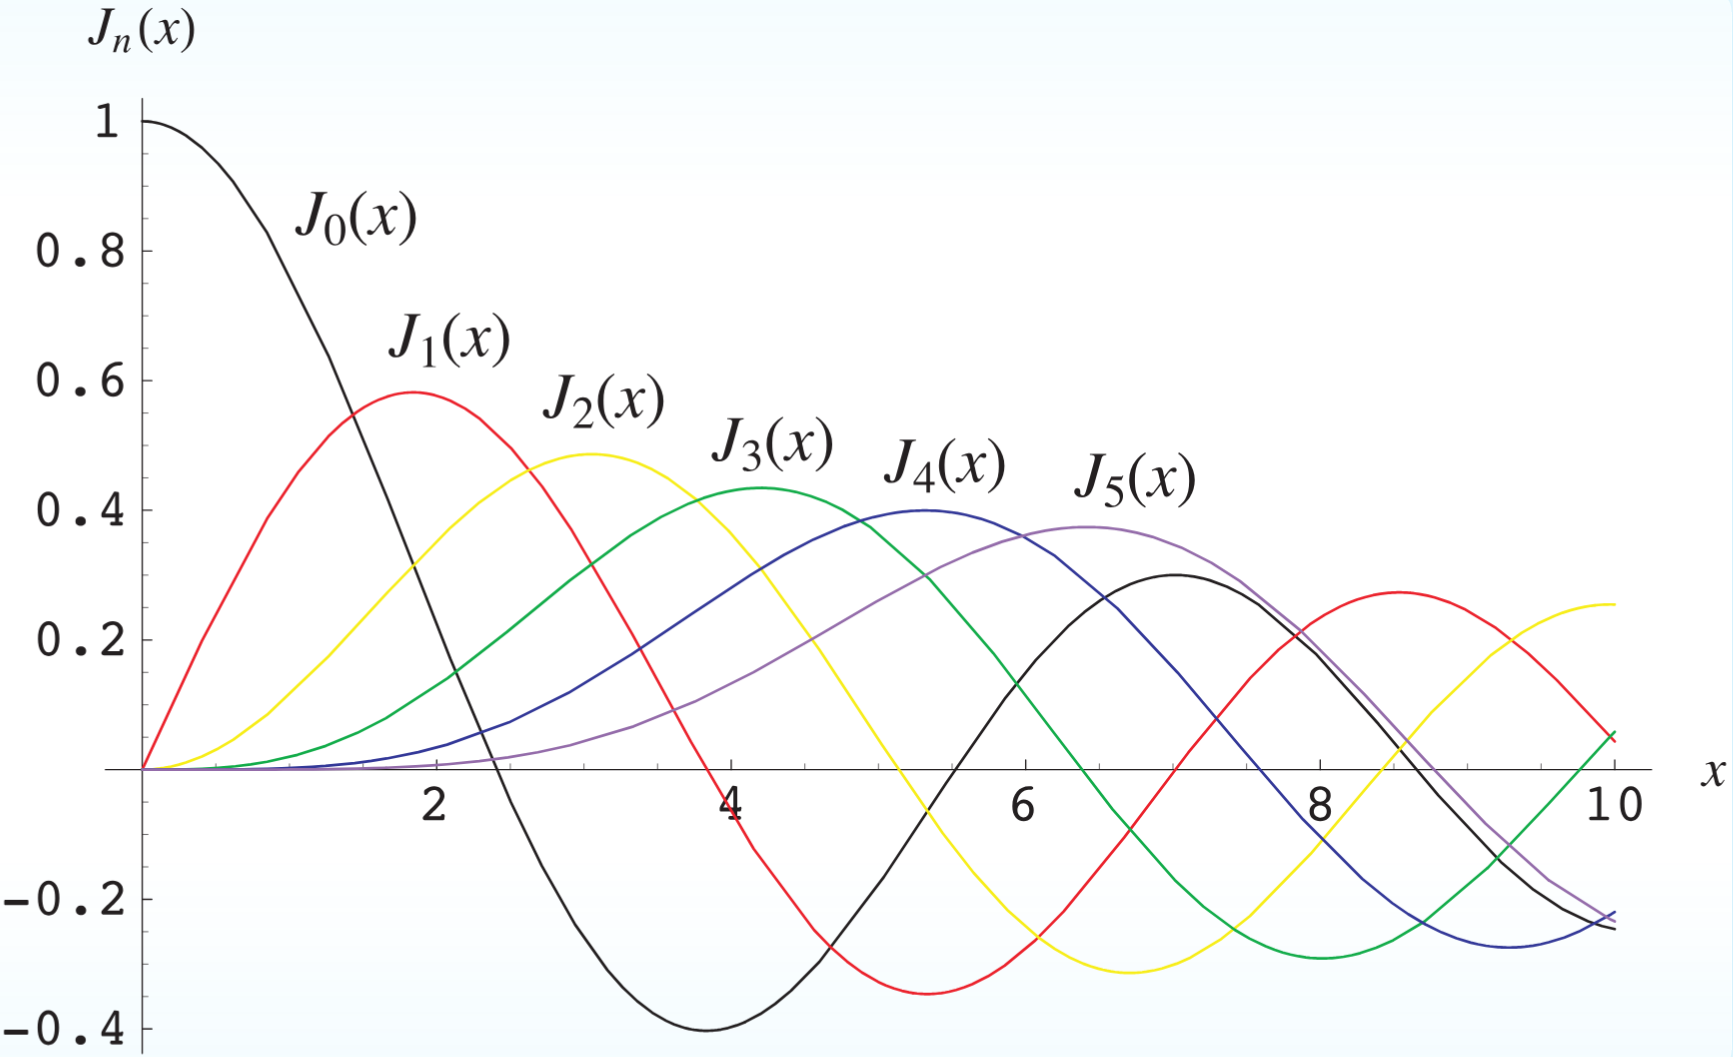
\includegraphics[width=0.6\textwidth]{Images/4.1.png}
    \caption{Graph of Bessel Function $J_0\bracket{x}$ and $J_1\bracket{x}$}
    \label{fig:4.1}
\end{figure}
\newpage
\subsection{Legendre's Equation}
\nicerbox{1}{
Another $2^{\text{nd}}$ order ODE that occurs frequently in STEM. Defined as:
\begin{equation}
    \bracket{1-x^2}y''-2xy'+k\bracket{k+1}y=0,\quad\text{where }k\in\mathbb{R}
\end{equation}
Solving using Frobenius method, the indicial equation gives $c=0$ and $c=1$. The two corresponding solutions are:
\begin{align}
    [c=0]:&\quad y_1=a_0\cbracket{1-\frac{k\bracket{k+1}}{2!}x^2+\frac{k\bracket{k-2}\bracket{k+1}\bracket{k+3}}{4!}x^4-\ldots}\\
    [c=1]:&\quad y_2=a_1\cbracket{x-\frac{\bracket{k-1}\bracket{k+2}}{3!}x^3+\frac{\bracket{k-1}\bracket{k-3}\bracket{k+2}\bracket{k+4}}{5!}x^5-\ldots}\\
    &\text{where $a_0$ and $a_1$ are arbitrary constants}\nonumber
\end{align}
The \textit{general solution} is thus $y=y_1+y_2$.
}\vspace{-3ex}
\subsubsection{Legendre Polynomials}
\begin{itemize}[\tiny$\bullet$]
    \item When $k\in\mathbb{Z}$ (integer), one of the solution's series will terminate after finite terms.
    \item The polynomial that is left, $P_n\bracket{x}$ is called \textbf{\textit{Legendre Polynomial.}}
    \item Constants $a_0$ and $a_1$ are chosen such that $P_n\bracket{x}$ has unit value, $\modulus{P_n\bracket{x}}=1$ at $x=1$.
    \item For example, to find $P_2\bracket{x}$:
    \begin{align*}
        [c=0]:\quad y&=a_0\cbracket{1-\frac{2\bracket{3}}{2!}x^2+\frac{2\bracket{2-2}\bracket{3}\bracket{6}}{4!}x^4+\ldots}\\
        &=a_0\cbracket{1-3x^2}
    \end{align*}
    When $a_0=-\frac{1}{2}$ and $x=1$, the value of $y=1$. Therefore:
    \begin{equation*}
        P_2\bracket{x}=-\frac{1}{2}\bracket{1-3x^2-1}
    \end{equation*}
\end{itemize}\vspace{-3ex}
\begin{figure}[!ht]
    \centering
    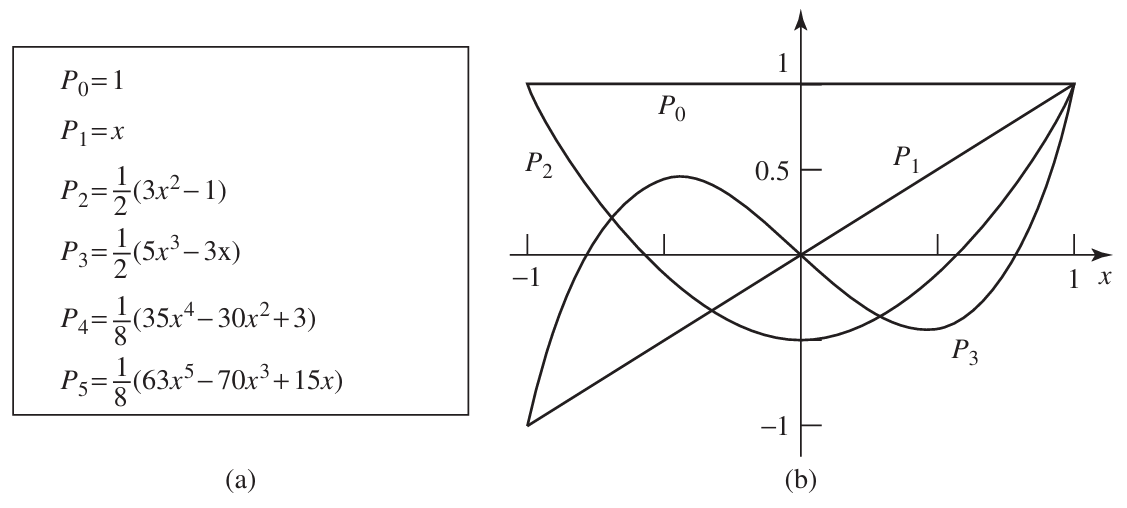
\includegraphics[width=0.65\textwidth]{Images/4.2.png}
    \caption{First few Legendre Polynomials, $P_n\bracket{x}$: (a) functional form, (b) graph }
    \label{fig:4.2}
\end{figure}
\newpage
\subsubsection{Rodrigue's Formula and the Generating Function}
\nicerbox{1}{
Legendre Polynomials can be derived by using \textbf{\textit{Rodrigue's Formula:}}
\begin{equation}
    P_n\bracket{x}=\frac{1}{2^nn!}\frac{d^n}{dx^n}\bracket{x^2-1}^n
\end{equation}
\textbf{\textit{Generating Function}} for Legendre Polynomials are useful to obtain values of $P_n\bracket{x}$.
\begin{equation}
    \frac{1}{\sqrt{1-2xt+t^2}}=\summation{n=0}{\infty}P_n\bracket{x}t^n,\quad \modulus{x}\leq1,\ \modulus{t}<1
\end{equation}
}
\begin{enumerate}
    \item $P_n\bracket{-1}$ is found by considering $g\bracket{-1,t}$. Setting $x=-1$, we have:
    \begin{equation*}
        g\bracket{-1,t}=\frac{1}{\sqrt{1+3t+t^2}}\equiv \summation{n=0}{\infty}P_n\bracket{-1}t^n=P_0\bracket{0}+P_1\bracket{x}t+P_2\bracket{x}t^2+P_3\bracket{x}t^3+\ldots
    \end{equation*}
    Using binomial expansion, we can expand $\mathcal{LHS}$:
    \begin{equation*}
        \frac{1}{\sqrt{1+3t+t^2}}=\frac{1}{1+t}=1-t+t^2-t^3+\ldots
    \end{equation*}
    Therefore, comparing these expansions:
    \begin{equation*}
        P_n\bracket{-1}=\bracket{-1}^n.
    \end{equation*}
    \item $P_n\bracket{0}$ is found by considering $g\bracket{0,t}$. Setting $x=0$, we have:
    \begin{equation*}
        g\bracket{0,t}=\frac{1}{\sqrt{1+t^2}}\equiv\summation{n=0}{\infty}P_n\bracket{0}t^n=P_0\bracket{0}+P_1\bracket{0}t+P_2\bracket{0}t^2++P_3\bracket{0}t^3\ldots
    \end{equation*}
    Using binomial expansion, we can expand the $\mathcal{LHS}$:
    \begin{equation*}
        \frac{1}{\sqrt{1+t^2}}=1-\frac{1}{2}t^2+\frac{3}{8}t^4-\frac{5}{16}t^6+\ldots
    \end{equation*}
    Therefore, comparing these expansions:
    \begin{equation*}
        P_{2n}\bracket{0}=\bracket{-1}^n\frac{\bracket{2n-1}!!}{\bracket{2n}!!}
    \end{equation*}
    where $n!!$ is the double factorial:
    \begin{equation*}
        n!!=\begin{cases}
            n\bracket{n-2}\ldots\bracket{3}1,& n>0,\ \text{odd},\\
            n\bracket{n-2}\ldots\bracket{4}2,& n>0,\ \text{even},\\
            1,& n=0,\ -1
        \end{cases}
    \end{equation*}
\end{enumerate}
\newpage
\subsubsection{Sturm-Liouville Systems}
\nicerbox{1}{
\textbf{\textit{Sturm-Liouville system}} is a boundary value problem that is described by DE of form:
\begin{equation}\label{eqn:4.30}
    \sbracket{p\bracket{x}y'}'+\sbracket{q\bracket{x}+\lambda r\bracket{x}}y=0,\quad\text{for }a\leq x\leq b\text{ and }r\bracket{x}>0
\end{equation}
where the boundary conditions can be written in the form
\begin{equation}
    a_1y\bracket{a}+a_2y'\bracket{a}=0\quad\text{and}\quad\beta_1y\bracket{b}+\beta_2y'\bracket{b}=0
\end{equation}
Solutions of such systems are in the form of an \textit{infinite sequence of} \textbf{\textit{eigenfunctions $\mathbf{y_n}$}}, each \textit{corresponding to} an \textbf{\textit{eigenvalue $\mathbf{\lambda_n}$}}, for $n=0,1,2,\ldots$
}

\noindent For example, consider DE: 
\begin{equation*}
    y''+\lambda y=0,\quad \text{for }0\leq x\leq5\xrightarrow[\text{conditions}]{\text{boundary}}\ y\bracket{0}=0,\ y\bracket{5}=0
\end{equation*}
The boundary equations imply:
\begin{align*}
    \alpha_1\cdot\bracket{0}+\alpha_2y'\bracket{0}=0\quad&\text{and}\quad\beta_1\cdot\bracket{0}+\beta_2y'\bracket{0}=0\\
    \therefore\alpha_2=0\quad&\text{and}\quad\therefore\beta_2=0
\end{align*}
Expand Equation \ref{eqn:4.30} and comparing it with given DE:
\begin{align*}
    &p\bracket{x}y''+p'\bracket{x}y'+\sbracket{q\bracket{x}+\lambda r\bracket{x}}\equiv y''+\lambda y=0\\
    &\therefore p'\bracket{x}=0\quad\text{and}\quad\therefore q\bracket{x}=0\quad\text{and}\quad \therefore r\bracket{x}=1
\end{align*}
To solve $y''+\lambda y=0$, use auxiliary equation $m^2+\lambda=0$, which gives us roots $m=i\pm\sqrt{\lambda}$. Therefore, the general solution is:
\begin{equation*}
    y=A\sin\sqrt{\lambda}x+B\cos\sqrt{\lambda}x
\end{equation*}
Applying boundary conditions $y\bracket{0}=0$:
\begin{equation*}
    y\bracket{0}=0=A\sin\bracket{0}+B\cos\bracket{0}\Longrightarrow B=0
\end{equation*}
Applying boundary conditions $y\bracket{5}=0$:
\begin{equation*}
    y\bracket{5}=0=A\sin\bracket{5\sqrt{\lambda}}\Longrightarrow \sqrt{\lambda}=\frac{n\pi}{5}\rightarrow\lambda=\frac{n^2\pi^2}{25}
\end{equation*}
There is $\infty$ number of eigenvalues, $\lambda$. The $n^{th}$ eigenvalue being denoted by $\lambda_n$ where $\displaystyle\lambda_n=\frac{n^2\pi^2}{25}$, with each eigenvalue having its corresponding eigenvector solution, $\displaystyle y_n=A_n\sin\frac{n\pi x}{5}$.
\newpage
\subsubsection{Orthogonality}
Two functions, $\f{x}$ and $\g{x}$ defined on interval $a\leq x\leq b$ are \textbf{mutually orthogonal} if:
\begin{equation}
    \intt{a}{b}\f{x}\g{x}dx=0
\end{equation}
Meanwhile, two functions are \textbf{mutually orthogonal} with \textbf{respect to the weight function} $w\bracket{x}$ if there's a \textit{third function $w\bracket{x}>0$ exists} such that:
\begin{equation}
    \intt{a}{b}\f{x}\g{x}w\bracket{x}dx=0
\end{equation}
An \textbf{important property} of the \textbf{solutions} to \textbf{Sturm-Liouville system} is that \textit{all solutions are mutually orthogonal with respect to weight function $r\bracket{x}$}.
\begin{equation}
    \intt{a}{b}y_m\bracket{x}y_n\bracket{x}r\bracket{x}dx=0,\quad (m\neq n)
\end{equation}
\subsubsection{Revisited Legendre's Equation}
All \textbf{Legendre Polynomials,} $P_n\bracket{x}$ are \textit{mutually orthogonal}:
\begin{equation}
    \intt{-1}{1}P_m\bracket{x}P_n\bracket{x}dx=0
\end{equation}
\textbf{\textit{Proof:}}\\
The equations $\bracket{1-x^2}y''-2xy'+n\bracket{n+1}y=0$ is Legendre's Equation and has Legendre Polynomials, $P_n\bracket{x}$ as solutions:
\begin{equation*}
    y_n=P_n\bracket{x},\quad\text{where }P_n\bracket{1}=1\text{ and }P_n\bracket{-1}=\bracket{-1}^n
\end{equation*}
This equation is an example of Sturm-Liouville system $\sbracket{p\bracket{x}y'}'+\sbracket{q\bracket{x}+\lambda r\bracket{x}}y=0$ with boundary conditions $a_1y\bracket{a}+a_2y'\bracket{a}=0\text{ and }\beta_1y\bracket{b}+\beta_2y'\bracket{b}=0$ where:
\begin{equation*}
    p\bracket{x}=1-x^2\quad\text{and}\quad q\bracket{x}=0\quad\text{and}\quad r\bracket{x}=1\quad\text{and}\quad \alpha_1,\alpha_2=1,0\quad\text{and}\quad\beta_1,\beta_2=1,0
\end{equation*}
Consequently, Legendre Polynomials $P_n\bracket{x}$ are mutually orthogonal when $m\neq n$.
\subsubsection{Polynomials as Finite Series of Legendre Polynomials}
\begin{itemize}[\tiny$\bullet$]
    \item Many DE cannot be solved analytically, so solution by power series is a powerful tool.
    \item \textbf{Any polynomial} can be \textit{written} in a \textit{finite series of Legendre Polynomials, $P_n\bracket{x}$}.
    \item Example 1: Show that $\f{x}=x^2$ can be written as a series of Legendre Polynomials.\\
    Assume that,
    \begin{align*}
        \f{x}&=x^2=\summation{n=0}{\infty}a_nP_n\bracket{x},\text{ then}\\
        x^2&=a_0P_0\bracket{x}+a_1P_1\bracket{x}+a_2P_2\bracket{x}+\ldots\\
        &=a_0\bracket{1}+a_1\bracket{x}+a_2\frac{3x^2-1}{2}+a_3\frac{5x^3-3x}{2}+\ldots
    \end{align*}
    Since $\mathcal{LHS}$ is a polynomial of $\text{degree}=2$, any Legendre Polynomial on $\mathcal{RHS}$ containing power of $x>2$ is excluded, i.e. $a_3=a_4=\ldots=0$. Therefore:
    \begin{equation*}
        x^2=a_0-\frac{a_2}{2}+a_1x+\frac{3}{2}a_2x^2\Longrightarrow a_2=\frac{2}{3},\ a_1=0,\ a_0-\frac{a_2}{2}=0\rightarrow a_0=\frac{1}{3}
    \end{equation*}
    Finally, we obtain an expression in terms of Legendre Polynomial, $P_n\bracket{x}$:
    \begin{equation*}
        x^2=\frac{1}{3}P_0\bracket{x}+\frac{2}{3}P_2\bracket{x}
    \end{equation*}
\end{itemize}
% \subsection{Hermite's Equation}
% Hermite polynomials are a sequence of orthogonal polynomials that are solutions to Hermite's equation:
% \begin{equation}
%     \frac{d^2y}{dx^2}-2z\frac{dy}{dx}+2ny=0
% \end{equation}
